\documentclass[conference]{IEEEtran}

\usepackage[colorlinks=true, linkcolor=blue, urlcolor=blue, citecolor=blue]{hyperref}
%\usepackage{natbib}
\usepackage{cite}
\usepackage{amsmath,amssymb,amsfonts}
\usepackage{algorithmic}
\usepackage{graphicx}
\usepackage{textcomp}
\usepackage{xcolor}
\usepackage{url}
\usepackage{float}
\usepackage{subcaption}
\usepackage{listings}

\def\BibTeX{{\rm B\kern-.05em{\sc i\kern-.025em b}\kern-.08em
    T\kern-.1667em\lower.7ex\hbox{E}\kern-.125emX}}
%\usepackage[T1]{fontenc}%

%\usepackage[no-math]{fontspec}
%   \setmainfont{Linux Libertine O}
%   \setsansfont{Linux Biolinum O}
%\usepackage{unicode-math}
%   \setmathfont{Asana Math}
\pagenumbering{arabic}

\pagestyle{plain}

\begin{document}
\title{Parallelization of classical molecular dynamics with OpenMP
\\
}
\author{\IEEEauthorblockN{Samuel Moerman}
\IEEEauthorblockA{\textit{Dept.\ of Computer Science} \\
\textit{New York University}\\
New York, USA \\
shm9853@nyu.edu}
\and
\IEEEauthorblockN{Anway Agte}
\IEEEauthorblockA{\textit{Dept.\ of Computer Science} \\
\textit{New York University}\\
New York, USA \\
ama10345@nyu.edu}
\and
\IEEEauthorblockN{Atmaj Koppikar}
\IEEEauthorblockA{\textit{Dept.\ of Computer Science} \\
\textit{New York University}\\
New York, USA \\
ark9238@nyu.edu}
\and
\IEEEauthorblockN{Mihir Prajapati}
\IEEEauthorblockA{\textit{Dept.\ of Computer Science} \\
\textit{New York University}\\
New York, USA \\
mp6507@nyu.edu}
}

\maketitle
\thispagestyle{plain}


\begin{abstract}
Molecular
dynamics is a computational technique that provides atomic-level insights into material and chemical compound behavior
by simulating interatomic interactions. This work presents a novel molecular dynamics engine with multicore parallelization
strategies for electrostatic, dispersion, and bonded interactions. 

The proposed parallelization approach for electrostatic and dispersion interactions utilizes Newton's third law of 
motion to symmetrize interaction calculations, effectively reducing the computational complexity by eliminating 
redundant pairwise interactions. Extensive benchmarking reveals performance improvements that scale with increased
thread count, highlighting the effectiveness of the proposed parallel decomposition strategy.
In contrast, the non-bonded interaction parallelization exhibited limited scalability, failing to achieve linear 
performance improvements with increasing system size. 

Additionally, a comprehensive analysis examines the cache locality and memory access patterns of the parallelization 
strategy, revealing insights into potential future thread-level performance optimization. Future work proposes exploring a 
hybrid CPU/GPU architecture using spatial decomposition techniques to further enhance performance and scalability.

\end{abstract}

\begin{IEEEkeywords}
Parallelization, OpenMP, Molecular Dynamics, Non-Bonded Interactions
\end{IEEEkeywords}

\section{Introduction}
Molecular dynamics (MD) is a computational technique that simulates the behavior of atoms and molecules by numerically 
solving their equations of motion. At its core, MD acts as a computational microscope, allowing researchers to 
observe and predict the dynamic behavior of molecular systems with at an atomic-level detail.


Molecular dynamics is based on the integration of Newton's equations of motion. For a system of N particles, this
 corresponds to the following equation:
\begin{align}
    m_i \frac{d^2\mathbf{r}_i}{dt^2} = \mathbf{f}_i = -\frac{\delta}{\delta \mathbf{r}_i}V(\mathbf{r}_1,\mathbf{r}_2,\ldots,\mathbf{r}_N)
\end{align}
Where $\mathbf{r}_1,\mathbf{r}_2,\ldots,\mathbf{r}_N$ represent the set of nuclear coordinates of the N-particle system, 
$V(\mathbf{r}_1,\mathbf{r}_2,\ldots,\mathbf{r}_N)$ the potential energy in function of these coordinates, $\mathbf{f}_i$
the force acting on particle $i$ and $m_i$ the mass of particle $i$. 

The MD simulation follows a systematic computational workflow. An initial system configuration is provided to
the program. Based on the initial positions of the particles in the system, the forces are calculated. 
These forces are then used to 
update each particle's position and velocity. These positions and velocities then form the input for the subsequent
timestep and the cycle repeats itself. It is in this way that the program iteratively determines the behavior of the 
system, utilizing numerical 
integration techniques, such as the Verlet algorithm.
This workflow is graphically represented in Fig.~\ref{fig:overview}

Since this forms a system of non-linear differential equations not solvable analytically, MD relies on numerical 
integration algorithms to iteratively calculate particle positions and speeds throughout time. The power of MD 
lies in its ability to generate a comprehensive trajectory showing how the molecular system evolves, providing 
insights into atomic-level phenomena that are challenging to observe experimentally.


% This forms a system of non-linear differential 
% equations, which is not solvable analytically. The simulations use a numerical integration algorithm to iteratively
% calculate the positions and speeds of the particles throughout time.~\cite{frenkel2001understanding}

% Some commonly used integration algorithms
% include Verlet integration or Langevin integration. More details on the numerical integration can be found in 
% the reference work of Daan Frenkel and Berend Smit.~\cite{frenkel2001understanding}

In this paper, the goal was to develop a comprehensive molecular dynamics (MD) simulation engine with a primary focus 
on parallel computational strategies. This encompassed the creation of a flexible and performant simulation framework 
capable of modeling interatomic interactions through the implementation of key physical force calculations, 
specifically targeting electrostatic, dispersion, and bonded interactions.

The core objectives of this work encompassed several important aspects of computational molecular dynamics and 
high-performance computing:
\begin{itemize}
    \item Engine Development: Design a modular molecular dynamics engine that can simulate fundamental interatomic 
    forces with computational efficiency and numerical precision. This involved creating a robust framework for 
    particle representation, force calculation, and system evolution.

    \item Parallelization Strategies: Explore and implement advanced parallel computing techniques to overcome the 
    computational complexity inherent in pairwise interaction calculations. By leveraging multicore processor 
    architectures, the research aimed to dramatically reduce computational time for large-scale molecular simulations.

    \item Performance Optimization: Develop parallelization approaches that not only distribute computational load 
    across multiple threads but also maximize cache utilization and minimize synchronization overhead. This required 
    a deep understanding of both computational algorithms and hardware-level performance characteristics.

    \item Comparative Analysis: Systematically benchmark the parallelization strategies for various interaction types, 
    critically evaluating their scalability, performance gains, and computational efficiency across different system 
    sizes.
\end{itemize}

% The motivation for this research came from the growing need for computationally efficient molecular dynamics
% simulations that can provide atomic-level insights into material behavior while managing the exponentially 
% increasing computational demands of larger and more complex systems.

By focusing on these objectives, the research sought to contribute to the ongoing advancement in computational 
physics, demonstrating innovative approaches to parallelizing complex scientific computing tasks and providing 
a flexible framework for future molecular dynamics investigations.

\begin{figure}[H]
    \centering
    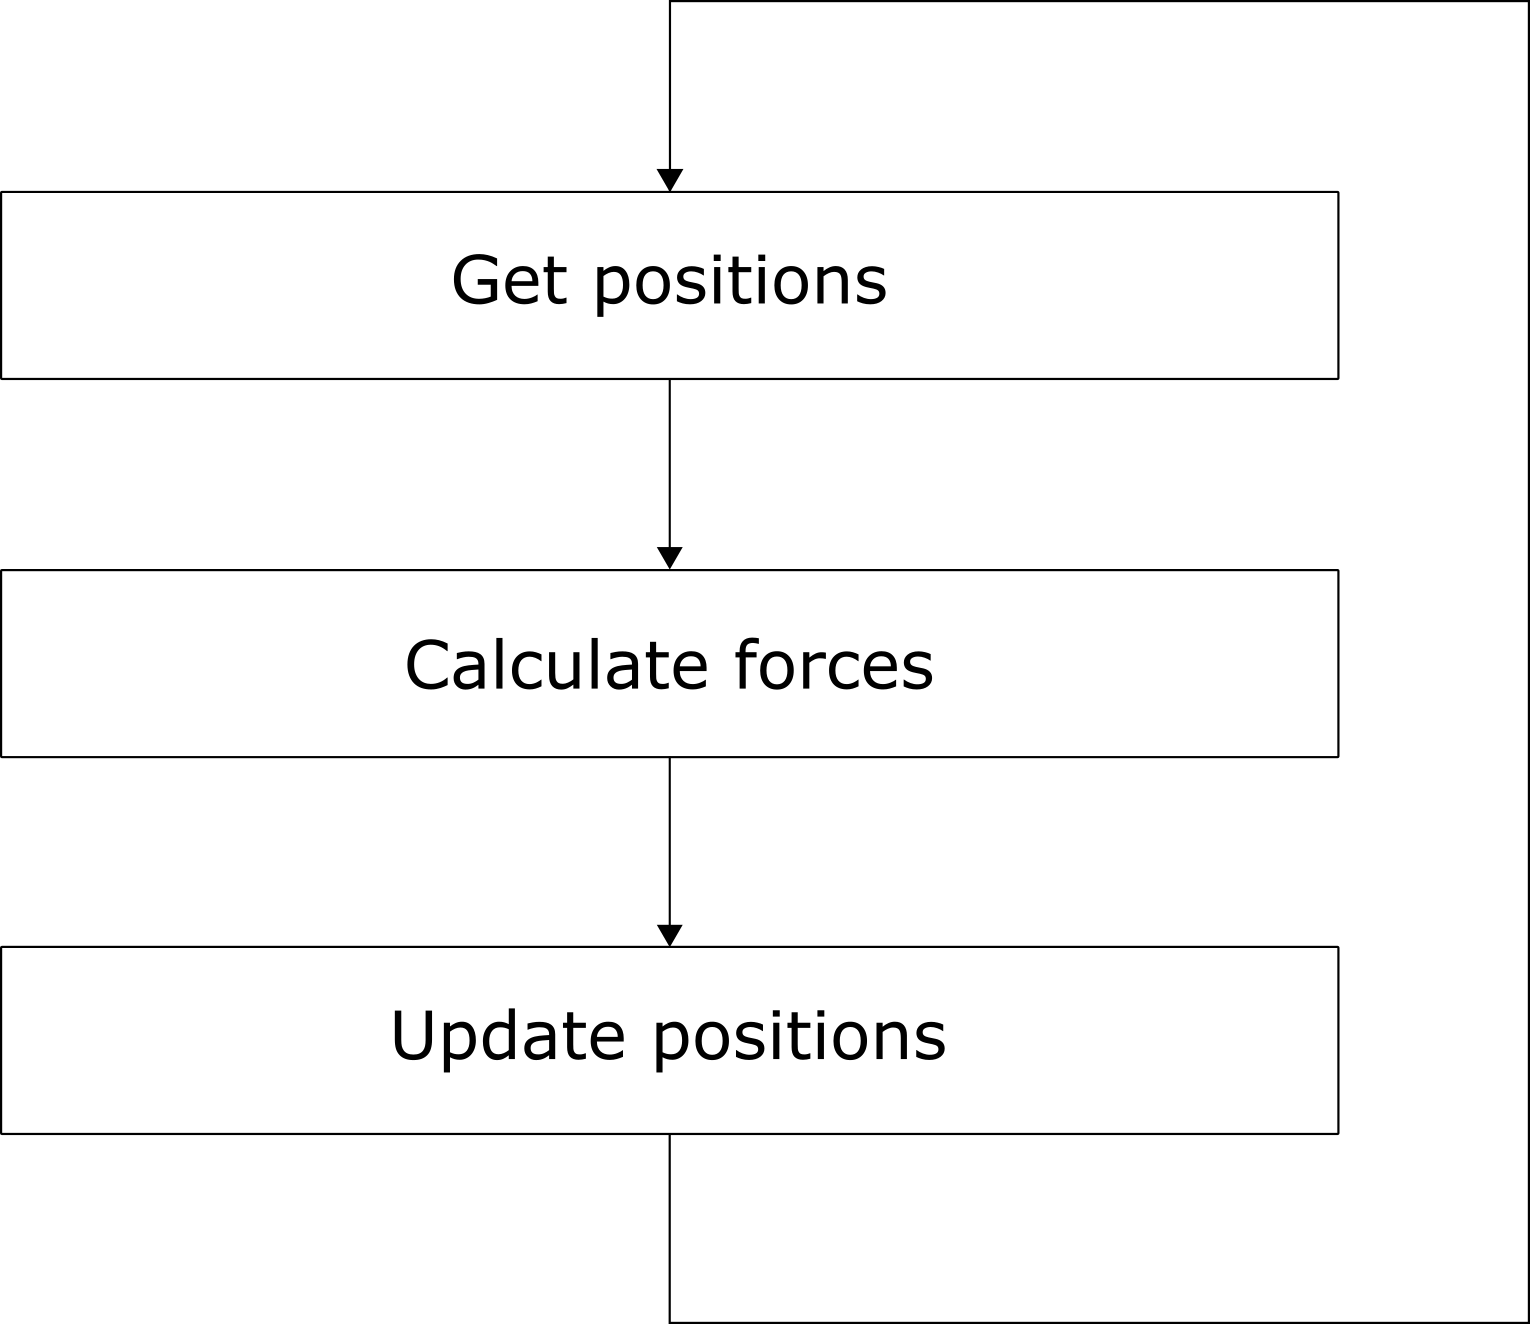
\includegraphics[width=0.7\linewidth]{images/verlet_concept.png}
    \caption{Conceptual visualization of the core concept behind molecular dynamics}\label{fig:overview}
\end{figure}


\section{Molecular Dynamics Engine}\label{md}

Organic molecules and biological macromolecules are typically described with the following expression:
\begin{equation}
    \begin{aligned}
    V(\mathbf{r}_1,\mathbf{r}_2,\ldots,\mathbf{r}_N) &= V_{\mathrm{bonds}} + V_{\mathrm{angles}} + 
                                                        V_{\mathrm{dihedrals}}\\
                                                    &+ V_{\mathrm{impropers}} + V_{\mathrm{dispersion \: interaction}}\\
                                                    &+ V_{\mathrm{electrostatic \: interaction}}
    \end{aligned}
\end{equation}
where $\mathbf{r}_1,\mathbf{r}_2,\ldots,\mathbf{r}_N$ are the particles in the system, $V$ is the potential energy of the
system in function of these particles, $V_{\mathrm{bonds}}$ the potential related to the bonds, $V_{\mathrm{angles}}$ 
the potential related to the angles, $V_{\mathrm{dihedrals}}$ the potential related to the dihedrals, 
$V_{\mathrm{impropers}}$ the potential related to the improper torsions, $V_{\mathrm{dispersion \: interaction}}$ 
the potential related to the dispersion interaction and $V_{\mathrm{electrostatic \: interaction}}$ the potential 
related to the electrostatic interaction. 

As described above, the formula consists of different types of potentials.
The term $V_{\mathrm{bonds}}$ can be described as follows:
\begin{equation}
    \begin{aligned}
    V_{\mathrm{bonds}} &= \sum_{\mathrm{bonds}} \frac{k_d}{2}*{(d-d_0)}^2
    \end{aligned}
\end{equation}
where $d$ is the distance between two particles, $d_0$ the standard bond distance for that particular combination of 
particles and $k_d$ the parameter associated with that specific bond. Not that this term is a sum of harmonic 
potentials. The energy increases as the bond distance deviates from the standard bond distance. When the bond 
distance reaches the standard bond distance, the energy associated with this bond becomes zero, which corresponds 
to a harmonic oscillator in a vacuum. The $k_d$ variable is part of the set of parameters specific to the 
forcefield as discussed above.

The term $V_{\mathrm{angles}}$ can be described in a similar way:
\begin{equation}
    \begin{aligned}
    V_{\mathrm{angles}} &= \sum_{\mathrm{angles}} \frac{k_{\theta}}{2}{(\theta-\theta_0)}^2
    \end{aligned}
\end{equation}
where $\theta$ represents the angle between a given set of 3 particles, $\theta_{0}$ the standard angle for this 
particular set and $k_{\theta}$ the parameter associated with that specific angle. The interpretation of this 
term is similar to $V_{\mathrm{bonds}}$, in that a deviation from the standard angle results in an increased energy.

A final term which is described by means of a harmonic oscillator is the term $V_{\mathrm{impropers}}$, which is 
often introduced to  maintain planarity of groups with a flat geometry or sometimes to preserve chirality:
\begin{equation}
    \begin{aligned}
    V_{\mathrm{impropers}} &= \sum_{\mathrm{impropers}} \frac{k_{\psi}}{2}{(\psi-\psi_0)}^2
    \end{aligned}
\end{equation}
where $\psi$ represents the angle between a set of 3 particles, $\psi_0$ the standard improper angle for that 
particular combination of particles and $k_{\psi}$ the parameter associated with that specific improper angle. 
Again, the interpretation is similar to $V_{\mathrm{bonds}}$, in that a deviation from the standard dihedral 
angle results in an increased energy.

The dihedral terms, also referred to as torsion terms, are responsible for introducing an energy barrier to the 
rotation of bonds which do not rotate freely. They can be expressed as follows:
\begin{equation}
    \begin{aligned}
    V_{\mathrm{dihedrals}} &= \sum_{\mathrm{dihedrals}} \frac{k_{\phi}}{2}(1+\cos(n\phi-\phi_0))
    \end{aligned}
\end{equation}
where $\phi$ represents the dihedral angle between a set of 4 particles, $\phi_0$ the standard dihedral angle for 
that particular set of particles, $k_{\phi}$ the parameter associated with that particular dihedral angle and $n$ 
the amount of minima in the rotational profile. The torsion terms are periodic in function of $\phi$ and are 
defined by two additional parameters, $n$ and $\phi_0$. Parameter $n$ refers to the number of minima in the 
rotational profile and is also known as the multiplicity of the function. The parameter $\phi_0$ is known as 
the phase factor, which determines the location of the minima. Often, the rotational profile of a dihedral 
function is not represented by one torsion function, but by a sum of multiple functions. 

The dispersion interaction $V_{\mathrm{dispersion \; interaction}}$ or van der Waals interaction is represented by 
the Lennard-Jones 12\-6 potential and can be rewritten as follows:
\begin{equation}
    \begin{aligned}
    V_{\mathrm{dispersion \; interaction}} &= \sum_{\mathrm{\substack{\mathrm{non-bonded} \\ \mathrm{pairs(i,j)}}}} 4\varepsilon_{ij}\left[
    {\left(\frac{\sigma_{ij}}{r_{ij}}\right)}^{12} - {\left(\frac{\sigma_{ij}}{r_{ij}}\right)}^6
    \right]
    \end{aligned}
\end{equation}
where $r_{ij}$ is the distance between a set of particles $(i,j)$, $\varepsilon_{ij}$ the maximum depth of the 
potential well for this set and $\sigma_{ij}$ the distance between this set where the interaction is zero. This 
interaction takes into account both the attractive and the repulsive aspect of non-bonded interaction. 

The electrostatic interaction $V_{\mathrm{electrostatic \; interaction}}$ is represented by Coulomb's law and can 
be rewritten as follows: 
\begin{equation}
    \begin{aligned}
    V_{\mathrm{electrostatic \; interaction}} &= \sum_{\mathrm{\substack{\mathrm{non-bonded} \\ \mathrm{pairs(i,j)}}}} \frac{q_i q_j}{4\pi\varepsilon_0r_{ij}}
    \end{aligned}
\end{equation}
where $r_{ij}$ is the distance between a set of particles $(i,j)$, $q_i$ and $q_j$ are the charges on particles $i$ 
and $j$ respectively and $\varepsilon_0$ the electric constant. In reality, charges are dispersed throughout a 
molecule. Many forcefields, however, calculate electrostatic interaction by using Coulomb's law, assuming all charges 
are static and can be represented as point charges. 

The Verlet integrator is a commonly used algorithm in molecular dynamics simulations to integrate Newton's equations 
of motion. It is favored for its numerical stability and time-reversibility properties. The positions of particles 
at time \( t + \Delta t \) are calculated based on their positions at time \( t \) and \( t - \Delta t \), along 
with the forces acting on them. The formula is given as follows:
\begin{align}
    \mathbf{r}_i(t + \Delta t) &= 2\mathbf{r}_i(t) - \mathbf{r}_i(t - \Delta t) + \Delta t^2 \cdot \frac{\mathbf{F}(t)}{m},
\end{align}

where \( \mathbf{r}(t) \) is the position of the particle at time \( t \), \( \Delta t \) is the integration time 
step, \( \mathbf{F}(t) \) is the force acting on the particle at time \( t \), and \( m \) is the particle's mass.

This method explicitly depends on the current and previous positions of the particle, eliminating the need to directly 
compute velocities. However, velocities can still be calculated as a midpoint approximation:

\begin{equation}
    \begin{aligned}
    \mathbf{v}(t) &= \frac{\mathbf{r}(t + \Delta t) - \mathbf{r}(t - \Delta t)}{2\Delta t}.
    \end{aligned}
\end{equation}

Because the Verlet algorithm calculates positions and approximates velocities at a single time step, it allows for 
efficient computation without sacrificing accuracy in simulations of large molecular systems.


\section{Literature Review}
    Molecular dynamics is a concept that is inherently very suited to parallelization. There are multiple
    MD engines that leverage parallelization, such as OpenMM.~\cite{eastman2010openmm} Because the forces that
    drive the behavior of the system are comprised of the sum of interactions between sets of particles, a parallelization
    can be performed over these interactions. Moreover, because the technique is inherently an approximative technique,
    there is lots of freedom to further optimize the calculations by using smart approximative algorithms. 
    In general, there are three main approaches that can be taken to improve the performance of the
    simulation engine. 
    % Spatial decomposition techniques split the simulation space up and improve performance by
    % processing these subregions in parallel. Force decomposition techniques are approximations based on physical grounds
    % that improve performance by reducing number of interaction pairs that need to be studied.

    \subsection{Atom Decomposition}
    In this approach, each of the $P$ processors are assigned a group of $N/P$ atoms. These atoms do not necessarily
    need to have any spatial or other relation to each other. However, in order to update the positions of the atoms
    in a processor $P_z$, it would require the positions of many atoms that are not contained in this processor
    $P_z$. This requires each processor to receive updated positions of all other atoms that are interacting with
    the atoms in $P_z$, in an operation referred to as all-to-all communication. This all-to-all communication incurs
    a cost of $O(N)$.~\cite{plimpton1995fast, fox1989solving}
    
    The atom decomposition algorithms
    spread the force calculations and integrations evenly across the processors. However, because of this global
    communication, the algorithm does not scale well with the number of particles in the system. The main advantage
    of these algorithms is their simplicity.~\cite{plimpton1995fast, fox1989solving}

    \subsection{Force Decomposition}
    % Force decomposition is based on the skew-symmetric force matrix arising from Newton's third law of motion. 
    In force decomposition approaches, each of the $P$ processors are assigned to a block of particle pairs (instead
    of particles themselves). In other words, the skew-symmetric force matrix $f$ that arises from Newton's third
    law of motion is spread out over the processors:
    \begin{align*}
        f =
        \begin{bmatrix}
        0 & f_{12} & f_{13} & \cdots & f_{1N} \\
        -f_{12} & 0 & f_{23} & \cdots & f_{2N} \\
        -f_{13} & -f_{23} & 0 & \cdots & f_{3N} \\
        \vdots & \vdots & \vdots & \ddots & \vdots \\
        -f_{1N} & -f_{2N} & -f_{3N} & \cdots & 0
        \end{bmatrix}  
    \end{align*}
    Each processor is responsible for a sub-block of $f$ of size $N/\sqrt{P} \times N/\sqrt{P}$. This is graphically
    illustrated in Fig~\ref{fig:force-decomp}
    \begin{figure}[H]
        \centering
        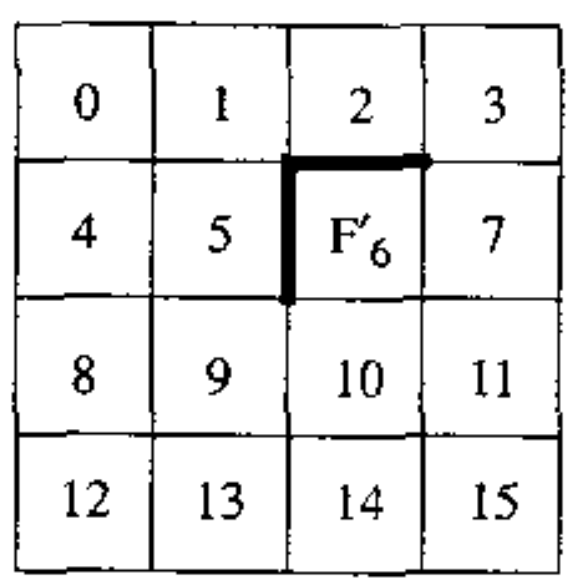
\includegraphics[width=0.35\linewidth]{images/force-decomp-graphic.png}
        \caption{Graphical representation of the force decomposition strategy. Modified 
        from Plimpton.~\cite{plimpton1995fast}}\label{fig:force-decomp}
    \end{figure}
    By permuting the force matrix $f$, the communication cost can be reduced from $O(N)$ to $O(N/\sqrt{P})$.
    Additionally, this method also does not require geometric information about the system being studies. In fact,
    to achieve better load balancing, it is better to randomize the atom ordering.~\cite{plimpton1995fast}



    \subsection{Spatial Decomposition Methods}

        \subsubsection{Domain Decomposition}
        Spatial decomposition methods are a fundamental approach to parallelizing MD simulations. The central idea is to 
        split the simulation region into boxes that are then independently processed. The volume of
        these boxes is chosen such that the load between the cores is optimally balanced. More modern approaches often
        tackle this issue in a dynamic fashion, by readjusting the boxes as the simulation progresses.


        Each of the processors is responsible for simulating the behavior of the particles in that region. One of the main
        challenges of this approach is how the interfaces between the subdivisions are handled. Many approaches
        leverage the fast multipole algorithm propsed by Greengard and Rothkin~\cite{greengard1987fast}. Other approaches
        could include the Barnes-Hut algorithm~\cite{barnes1986hierarchical}. These spatial decomposition 
        techniques are highly suited to CPU parallelization because of the irregular branching, adaptive recursion and 
        non-uniform memory
        access patterns. 

        \subsubsection{Neighbor Lists}
        Neighbor list is another spatial decomposition approach that can be used to parallelize MD simulations. The
        core idea is to maintain a list of potential interaction partners for each particle in the system. This
        significantly reduces the time complexity, given that the algorithm no longer needs to iterate over all
        atom pairs ($O(N)$), but only needs to iterate over the neighbor list for each particle ($O(N)$). These
        techniques are especially relevant for short-range non-bonded interactions. This technique is especially
        suited to CPU, given that it is extremely challenging to coalesce the memory, which is required for efficient
        GPU parallelization.~\cite{allen2017computer,verlet1967computer}



\section{Parallelization}\label{par}
The proposed parallelization approach sets out to parallelize the force calculations for the involved particle pairs.
A directed acyclic graph of the process that is being parallelized is represented in Fig.~\ref{fig:dag}
\begin{figure}[H]
    \centering
    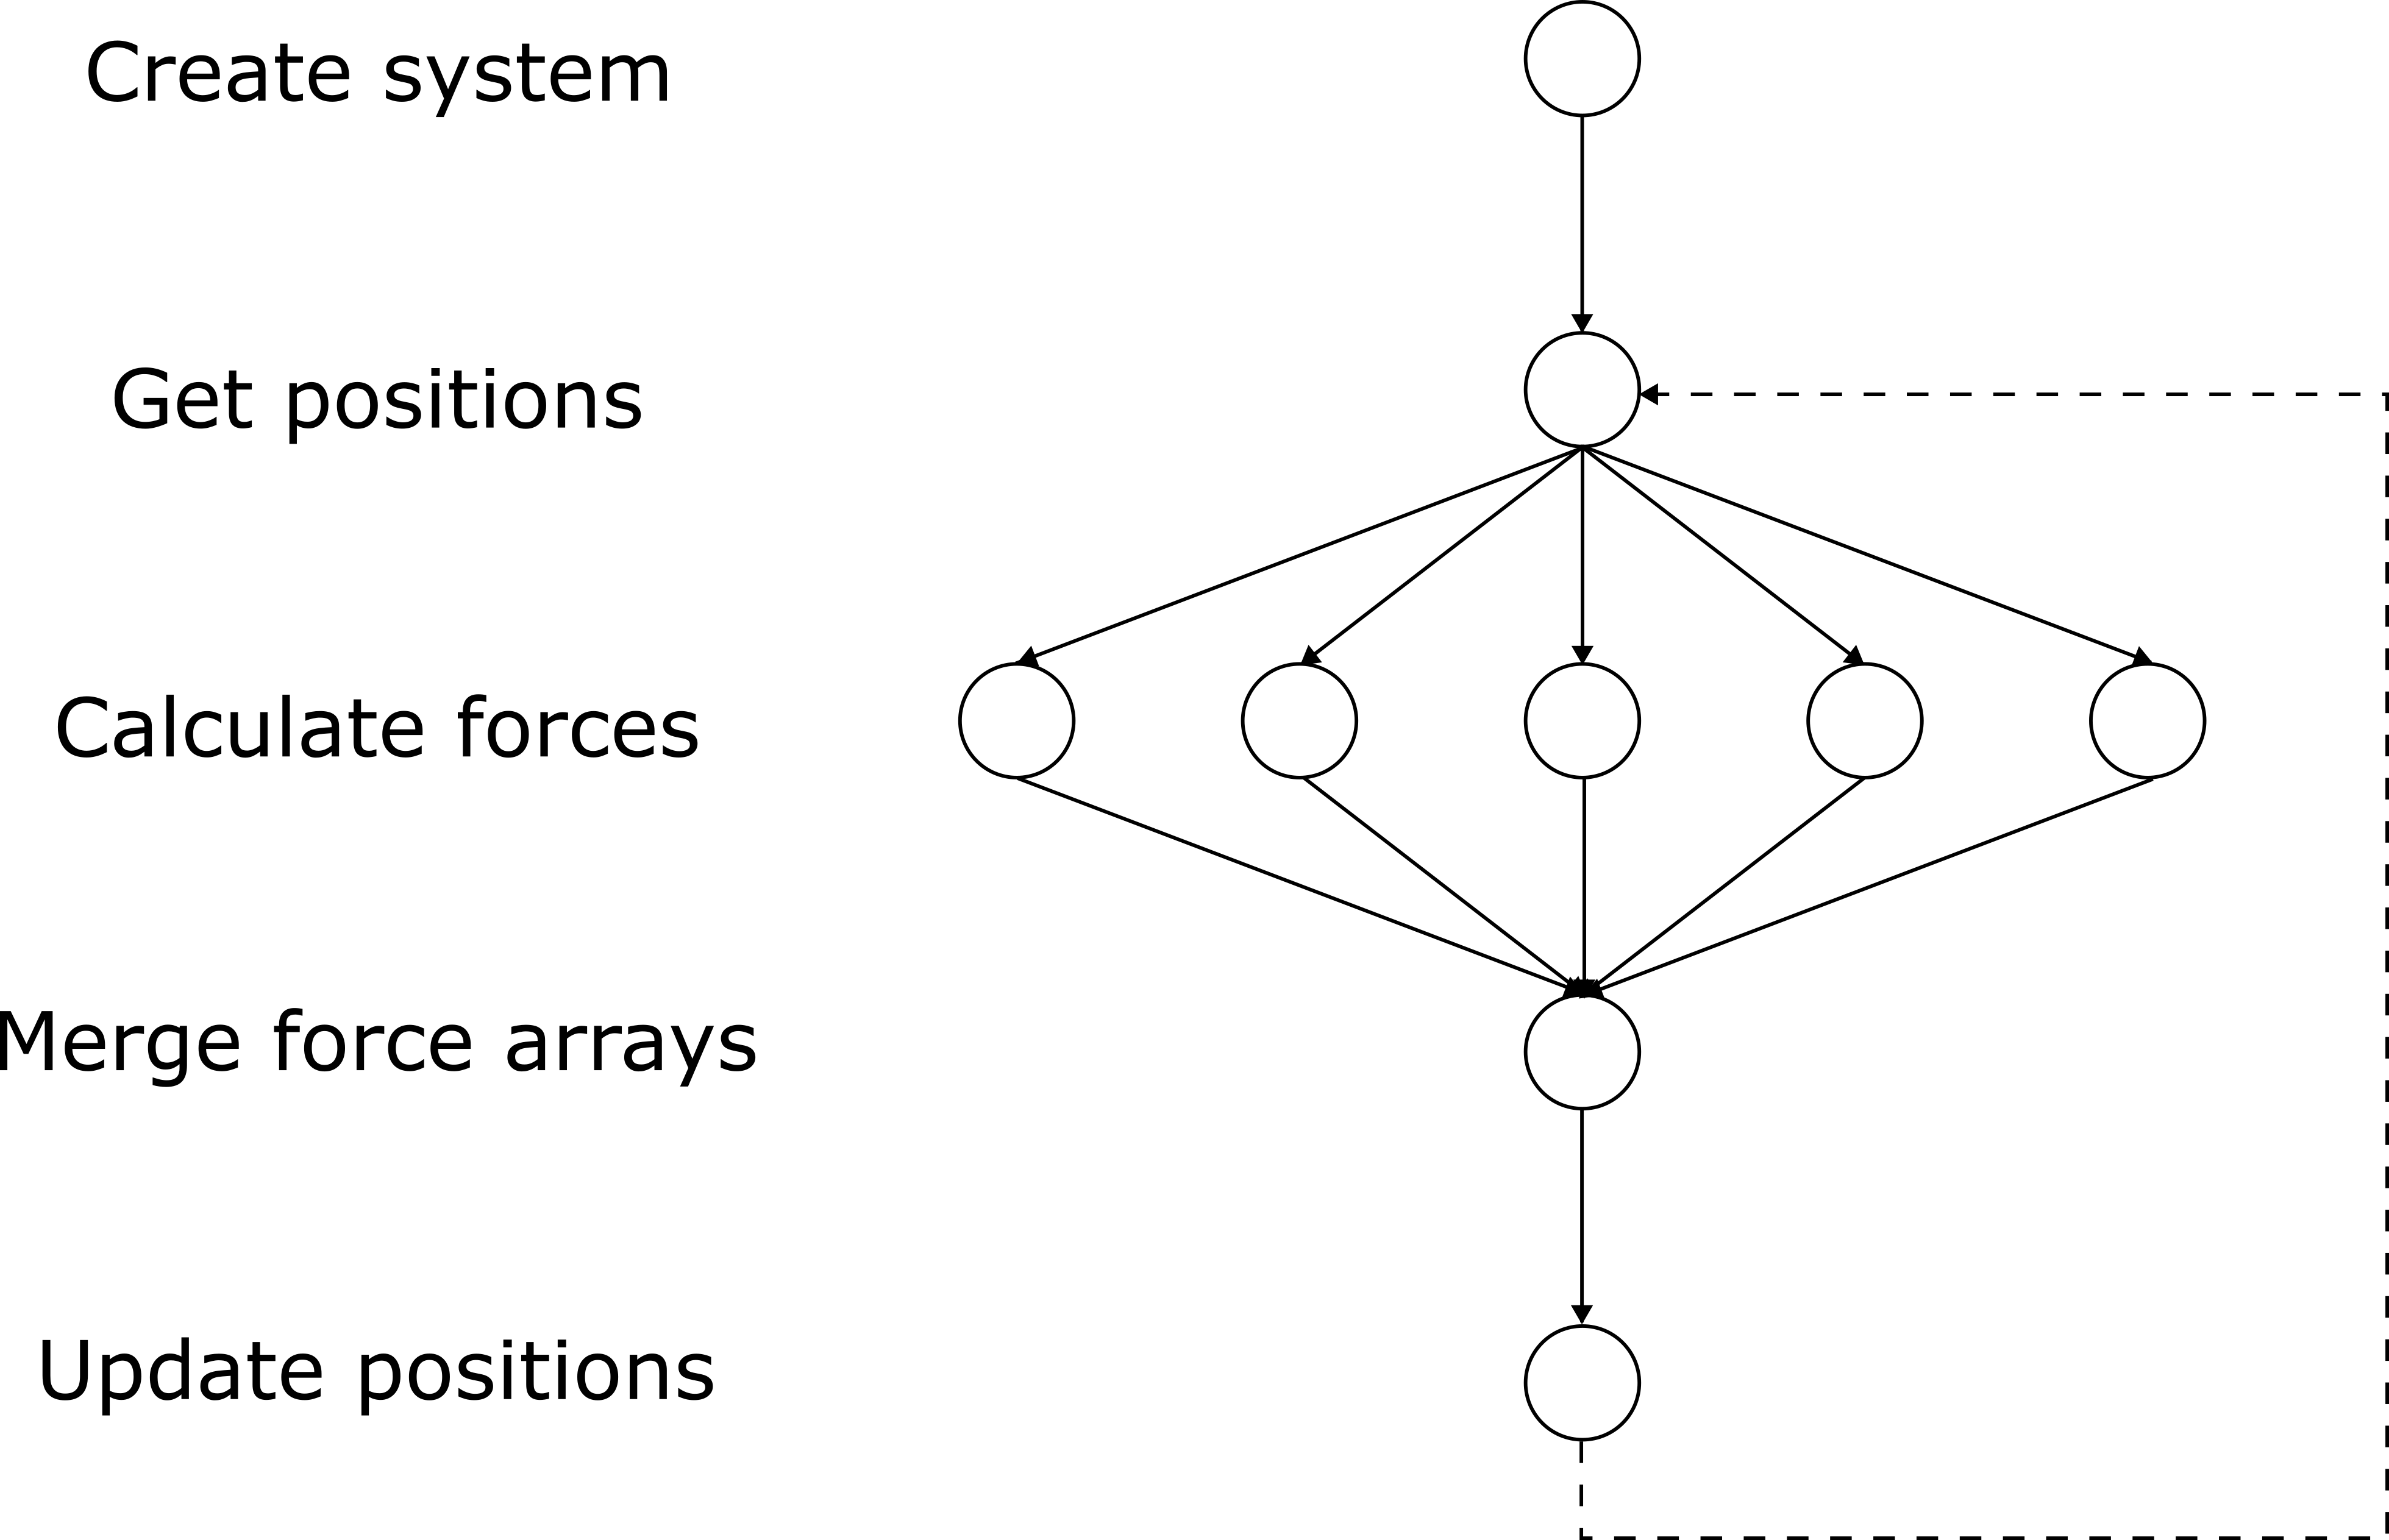
\includegraphics[width=\linewidth]{./images/dag.png} % This creates a placeholder box with text
    \caption{A direct acyclic graph illustrating the computations performed in the parallelized section of the code.
    Note that the dashed line illustrates that this DAG is executed for multiple timesteps to simulate the 
    behavior of the system.}\label{fig:dag}
\end{figure}

\subsection{Electrostatic Forces}
In general, the non-bonded interactions (i.e.\ the electrostatic interaction and the dispersion interaction) usually
take up the majority of the time for classical molecular dynamics simulations. This is because these interactions are
two-particle interactions, which would naively require a double loop over all particles resulting in an $O(N^2)$
time complexity. 
\begin{lstlisting}
    compute(system):
        for particles in system:
            for particles in system:
                - calculate distance
                - compute electrostatic 
                  force
    \end{lstlisting}


However, because of Newton's third law of motion, it is possible to leverage the concept of a skew-symmetric 
force matrix $f$
\begin{align*}
        f =
        \begin{bmatrix}
        0 & f_{12} & f_{13} & \cdots & f_{1N} \\
        -f_{12} & 0 & f_{23} & \cdots & f_{2N} \\
        -f_{13} & -f_{23} & 0 & \cdots & f_{3N} \\
        \vdots & \vdots & \vdots & \ddots & \vdots \\
        -f_{1N} & -f_{2N} & -f_{3N} & \cdots & 0
        \end{bmatrix}  
\end{align*}
of which only the upper or lower triangular portion needs to be calculated.
\begin{lstlisting}
compute(system):
    for particle pairs in system:
            - calculate distance
            - compute electrostatic force
\end{lstlisting}

This loop is parallelized using a
\verb|collapse(2)| clause, which can deal with non-rectangular loops since OpenMP 5.1.
\begin{lstlisting}
compute(system):
    #pragma omp for collapse(2)
    for particle pairs in system:
            - calculate distance
            - compute electrostatic force
            - store in local force vector

    #pragma omp critical
    - merge local force arrays
\end{lstlisting}

Note that thread-local force vectors are used during the calculations.

Because this loop is collapsed, the work across the iterations is uniform. Therefore, no schedule was needed to 
obtain optimal performance (which is not possible either way with a collapsed non-rectangular loop). Alternative setups 
with a schedule were also attempted, but the collapsed loop gave the best performance.

\subsection{Dispersion Forces}
This force type follows the same scheme as the electrostatic forces.

\begin{lstlisting}
compute(system):
    #pragma omp for collapse(2)
    for particle pairs in system:
            - calculate distance
            - compute dispersion force
            - store in local force vector

    #pragma omp critical
    - merge local force vectors
\end{lstlisting}

\subsection{Bonded Forces}
The bonded forces represent the bonds between two particles. They are created at the system creation stage, and are
stored in an \texttt{std::vector}. Besides this, the local force array concept is maintained from the non-bonded
forces.
\begin{lstlisting}
compute(system):
    #pragma omp for
    for bonds:
        - calculate distance between 
            particles in bond
        - compute dispersion force
        - store in local force vector

    #pragma omp critical
    - merge local force vectors
\end{lstlisting}
Again, because of the uniform work across all the iterations of the loops, introducing a schedule did not result in
an increased performance due to the additional overhead.

\section{Results}\label{res}
In this section, the results of the parallelization strategies will be reported. The benchmarking was performed on the
Crunchy 1 server, which contains a Four AMD Opteron 6272 (2.1 GHz) processor with 64 cores. Additionally, 256 GB of
memory is available. All measurements were performed in triplicate and averaged out. In order to 
make a fair assessment of the parallelization, this speedup is calculated relative to a proper sequential version
of this code rather than a parallel version run with a single thread. This way, overhead associated with ensuring
thread-safe memory access is also eliminated and the true performance of parallelization can be accurately assessed.

In the following subsections, plots of the speedup in regard to the number of threads will be given. These results
will then be discussed in Section~\ref{discussion}
Note that the x-axis of these plots is in a logarithmic scale, to represent the speedup over the full
range of threads in a clear manner.

    \subsection{Electrostatic Interaction}
    In Fig.~\ref{fig:electro-speedup}, a plot of the speedup of the electrostatic force calculations 
    in regard to the number of threads is displayed for a range of different system sizes.
    \begin{figure}[H]
        \centering
        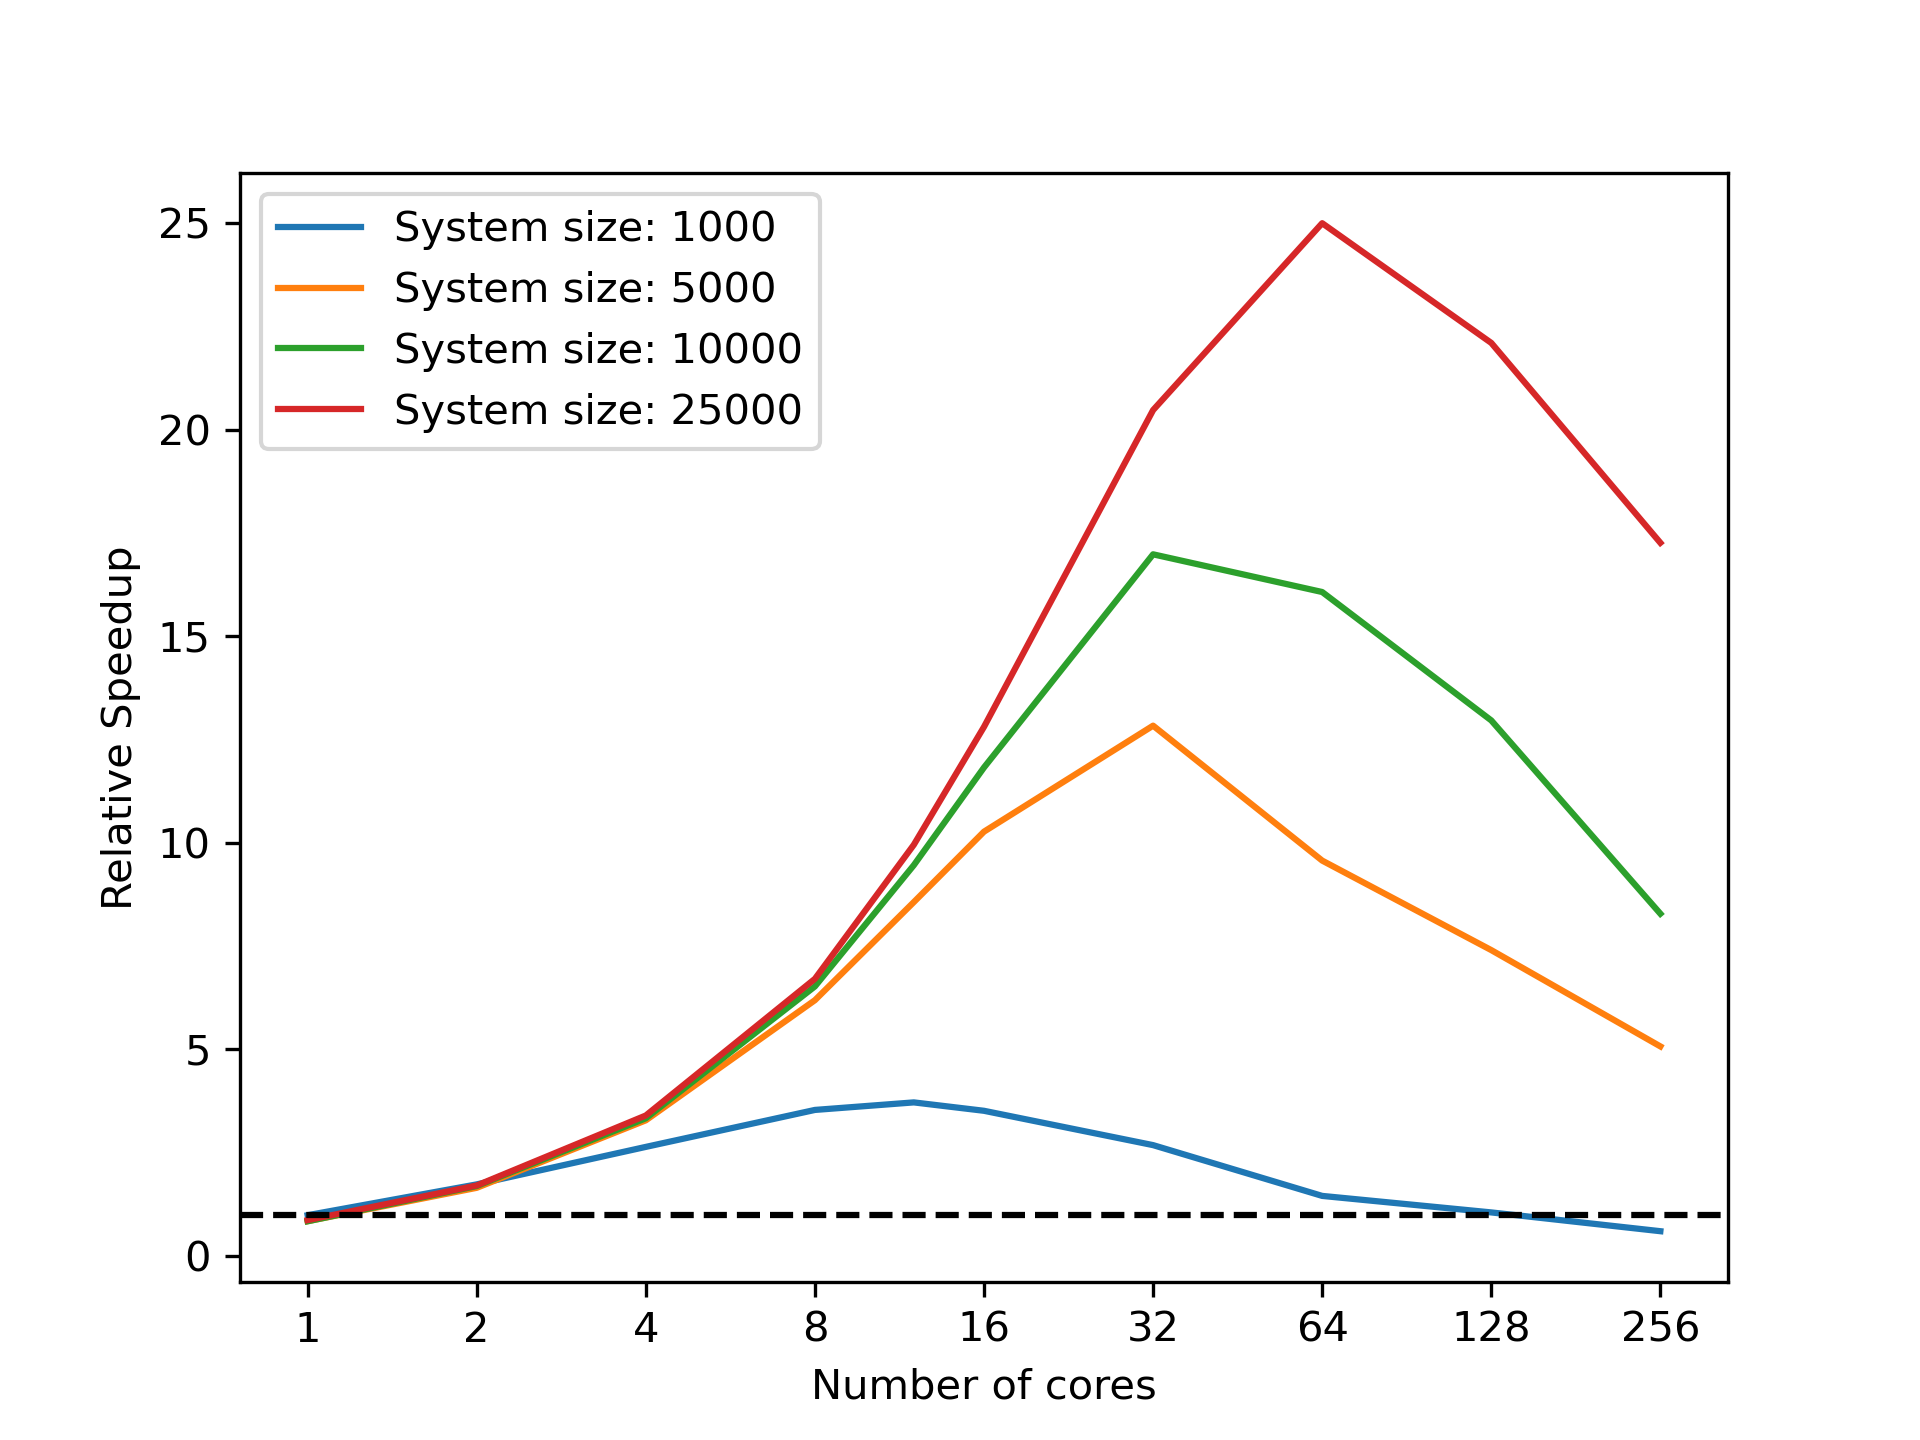
\includegraphics[width=\linewidth]{./images/electrostatic_scaling.png} % This creates a placeholder box with text
        \caption{Speedup of a range of systems containing only electrostatic interaction in function of the number 
        of threads}\label{fig:electro-speedup}
    \end{figure}
    A clear speedup can be observed for all system sizes. For the smallest system sizes, a speedup is achieved by leveraging
    multiple cores. However, this behavior only holds to a certain number of cores, after which there is a decrease
    in the speedup to the point where the sequential version becomes more performant. When increasing the system
    size, the parallelization is more scalable. In other words, more cores can be leveraged to achieve an even
    greater speedup. For the largest system size of $25000$, the maximum speedup corresponds to the $64$ logical
    cores that are available in the testing system. However, increasing the number of cores beyond this number
    also decreases performance.

    Additionally, some manual benchmarking was done to calculate the time spent per individual interaction. This
    seemed to be quite independent of the system size, and resulted in a maximum time spent on an interaction 
    around $400 ns$.

    \subsection{Dispersion Interaction}

    In Fig.~\ref{fig:dispersion-speedup}, a plot of the speedup of the electrostatic force calculations 
    in regard to the number of threads is displayed for a range of different system sizes.
    \begin{figure}[H]
        \centering
        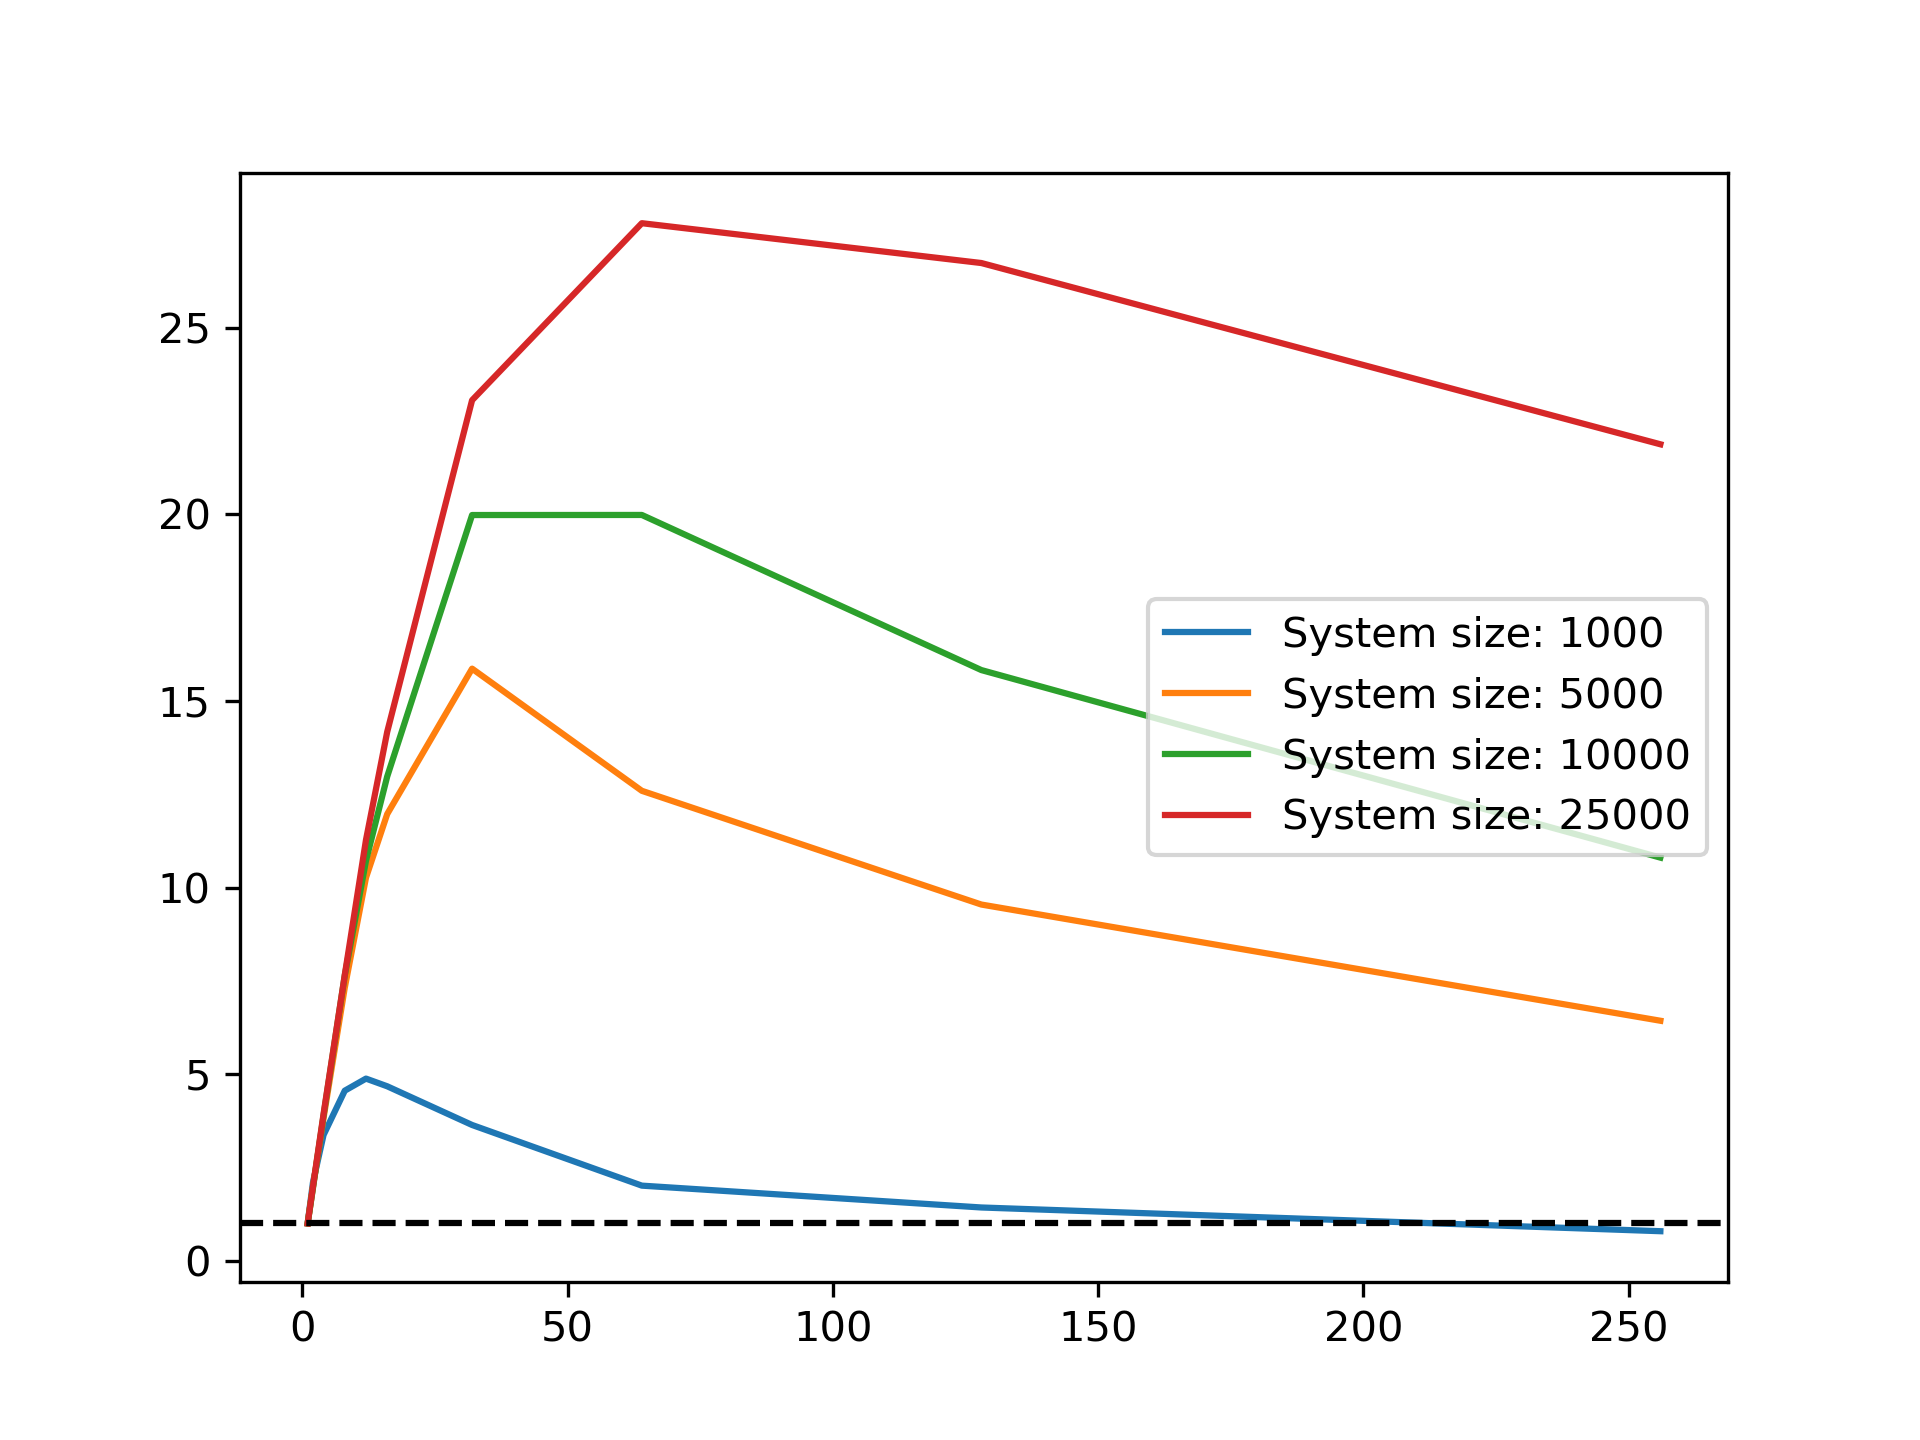
\includegraphics[width=\linewidth]{./images/dispersion_scaling.png} % This creates a placeholder box with text
        \caption{Speedup of a range of systems containing only dispersion interaction in function of the number 
        of threads.}\label{fig:dispersion-speedup}
    \end{figure}

    The trends for the dispersion interaction are largely similar to the electrostatic interactions, given that
    they iterate over the same interaction pairs. However, the maximum obtained speedup seems to be slightly
    larger than the electrostatic interactions.

    Additionally, some manual benchmarking was done to calculate the time spent per individual interaction. This
    seemed to be quite independent of the system size, and resulted in a maximum time spent on an interaction 
    around $400 ns$. Note that despite the increased complexity of this calculation, the time is more approximately
    equal to that of an electrostatic interaction.

    \subsubsection{Bonded Interaction}
    In Fig.~\ref{fig:bonded-speedup}, a plot of the speedup of the electrostatic force calculations 
    in regard to the number of threads is displayed for a range of different system sizes. In 
    Fig~\ref{fig:bonded2-speedup}, a similar benchmark is displayed, but for larger system sizes and smaller
    number of threads.

    \begin{figure}[H]
        \centering
        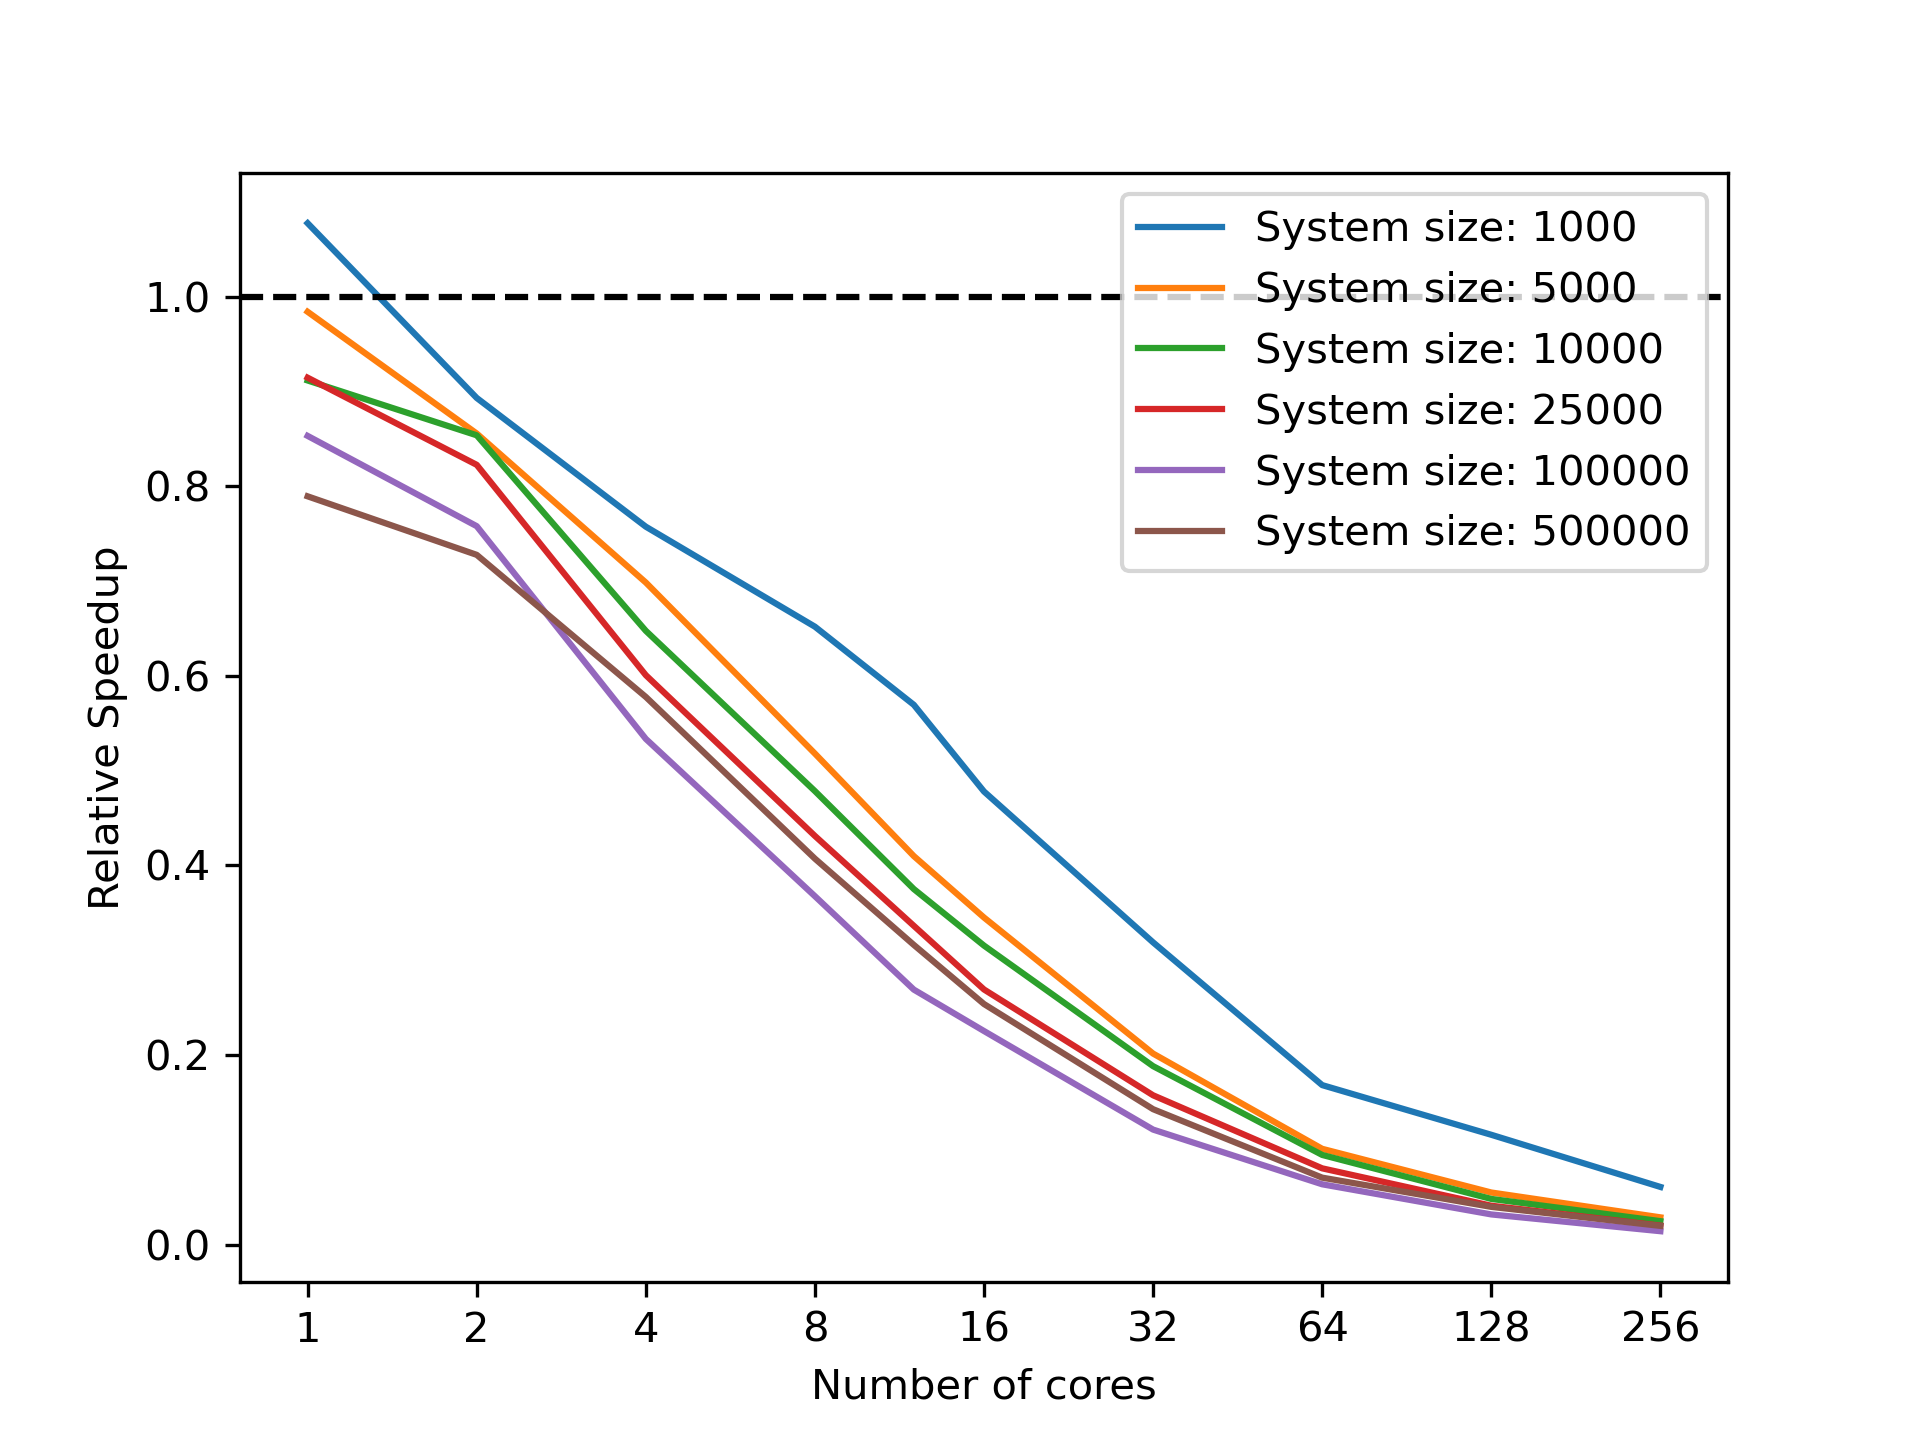
\includegraphics[width=\linewidth]{./images/bonds_scaling.png} % This creates a placeholder box with text
        \caption{Speedup of a range of systems containing only bonded interaction in function of the number 
        of threads.}\label{fig:bonded-speedup}
    \end{figure}
    \begin{figure}[H]
        \centering
        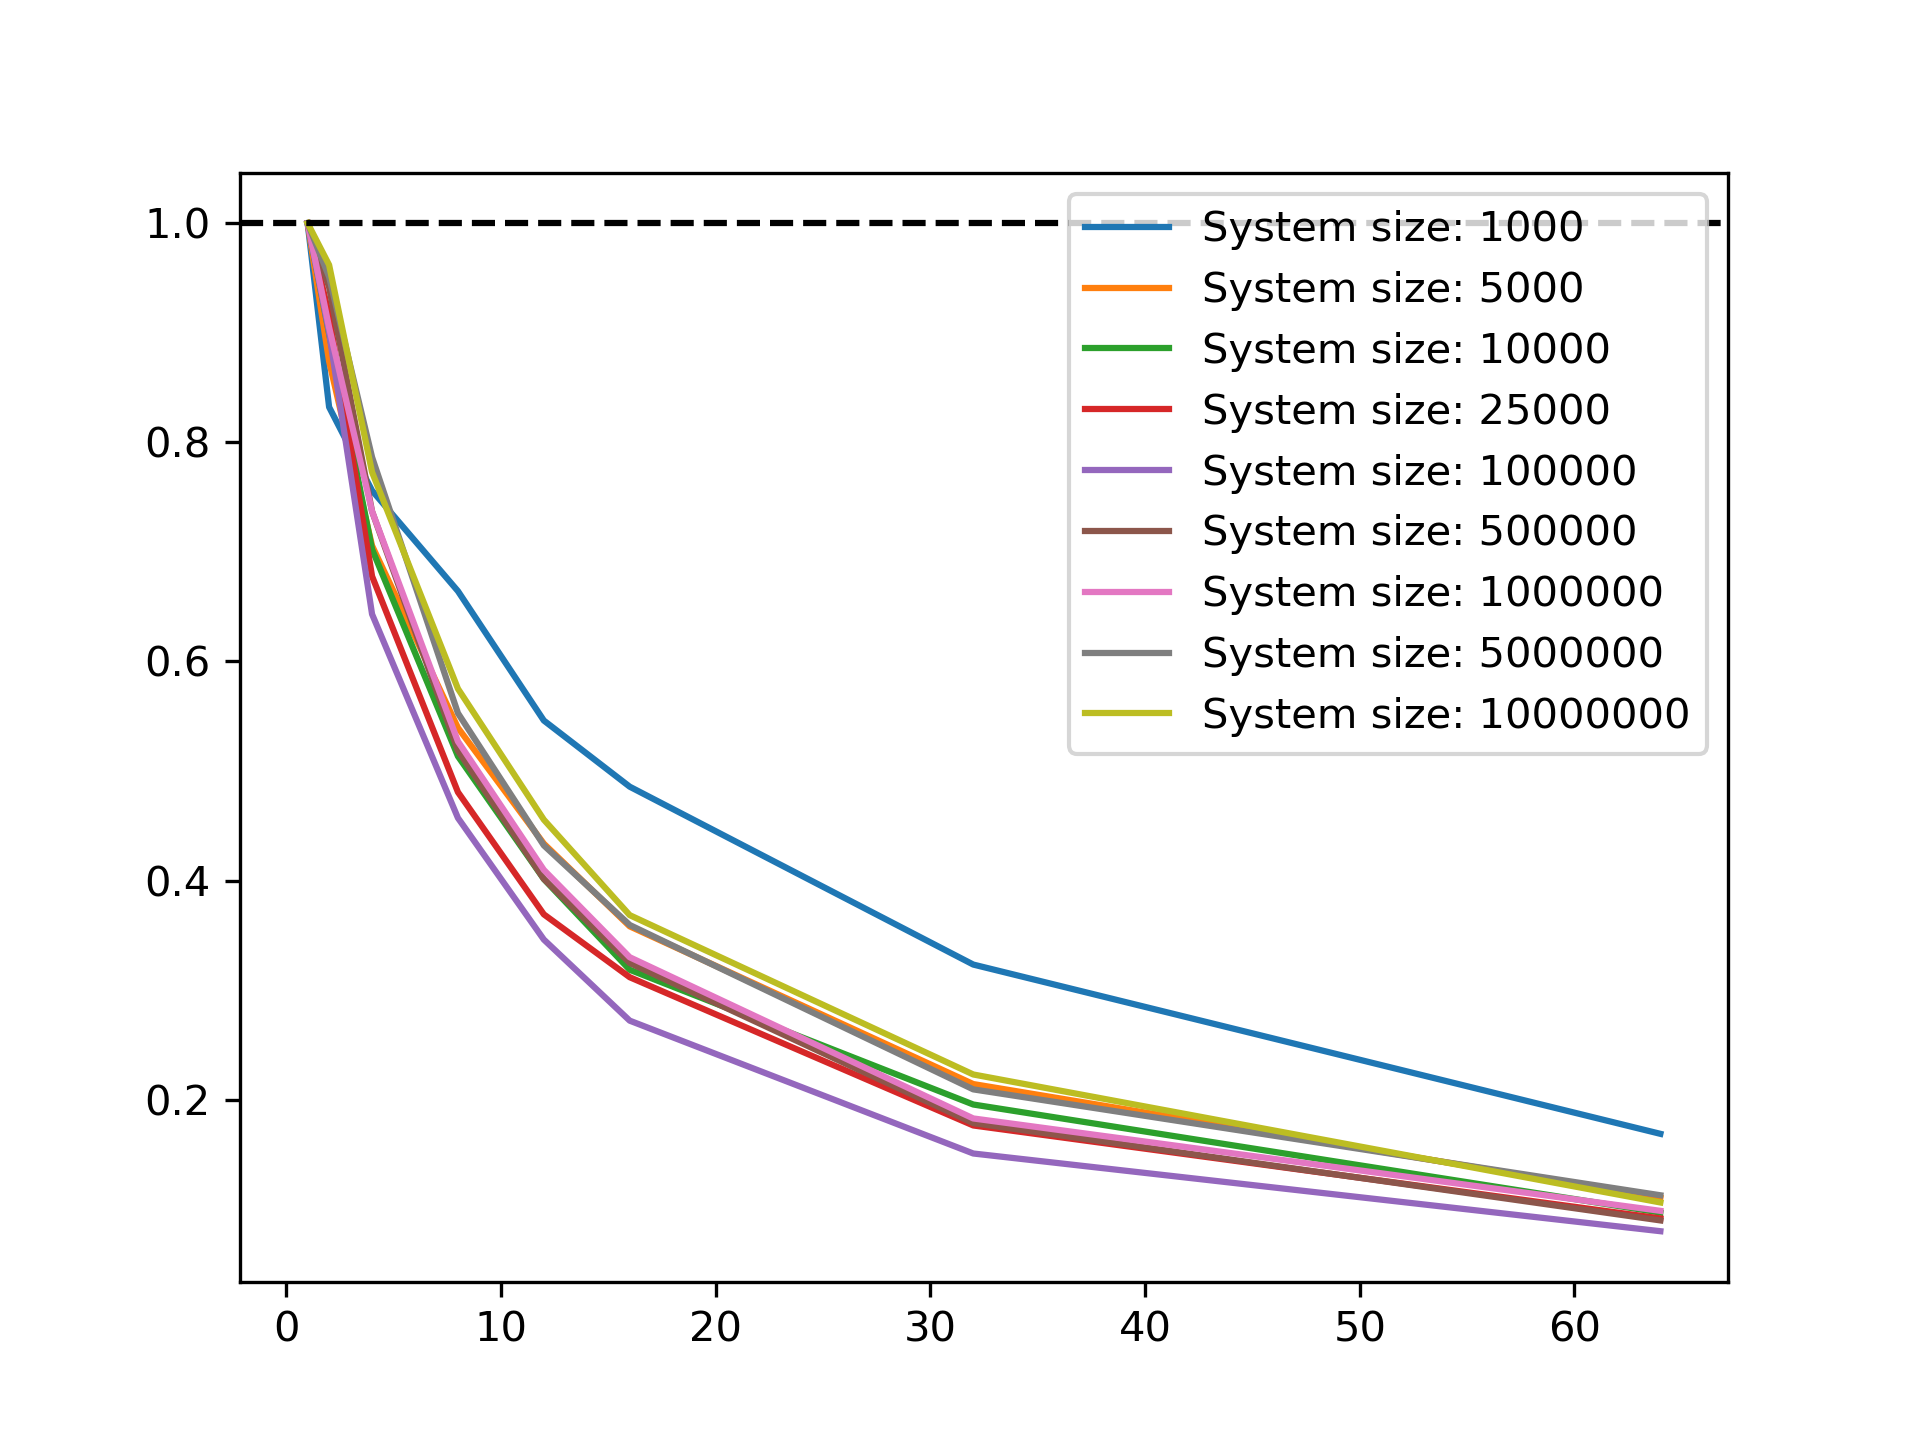
\includegraphics[width=\linewidth]{./images/bonds2_scaling.png} % This creates a placeholder box with text
        \caption{Speedup of a range of systems containing only bonded interaction in function of the number 
        of threads.}\label{fig:bonded2-speedup}
    \end{figure}

    Here we see no significant performance increase for the parallelization of the bonded forces. There is no
    clear trend over the system sizes, but we can note that the smaller system sizes seem to drop in performance
    slightly less steeply than the larger system sizes.

    % Additionally, some manual benchmarking was done to calculate the time spent per bond. This
    % seemed to be quite independent of the system size, and resulted in a maximum time spent on a single bond 
    % around $1000 ns$. Note the similarity of the calculation time with the other force types.

\section{Discussion}\label{discussion}
\subsection{Non-bonded Interactions}

Leveraging the skew-symmetric
force matrix, it is possible to eliminate a large section of the particle pairs that normally would be iterated
over. However, this results in a non-rectangular loop, which normally would not result in a uniform load balance.
However, because of the \verb|collapse(2)| cause, a uniform load balance is achieved after all. This was also
clearly observed during the development stage, where the timings for all threads were very uniform.

We can clearly see the best speedup and scaling for non-bonded interactions (i.e.\ the electrostatic forces and 
the dispersion forces). This is because of the collapsed double loop, which drastically increases the amount of
work per thread. As illustrated in Fig~\ref{fig:dispersion-speedup} and Fig~\ref{fig:electro-speedup}, small system
sizes only experience a speedup up to a limited number of cores. This is because a balance has to be found between
the overhead associated with managing multiple threads and the performance gain. As the number of cores is increased,
the overhead increases to the point where there is no performance gain with regard to the sequential code. As the
system size is increased, the amount of work that can be split over the threads also increases. Subsequently, the
overhead associated with managing these threads is also spread out more. This is the reason why the larger system
sizes experience performance gains for a larger number of threads. Note that the number of threads that correspond
to the largest performance gain corresponds to the number of logical cores in the system. Beyond this point, the
parallelism does not really increase anymore, because only concurrency is achieved.

As stated in Section~\ref{par}, the non-bonded force calculations make use of local force vectors to store the
calculated forces per thread. Subsequently, a critical section is used to merge these local force vectors
into the global vector. This was done for correctness and optimization purposes. It is entirely possible that two threads
are working on two separate interactions that happen to involve a common particle (e.g.\ forces $f_{ij}$ and $f_{ik}$ both 
involving particle $i$). If these two were to write to the global force vector, this would result in a race condition
and an incorrect end result. In these physical simulations, that is of course unacceptable. To mitigate this, a
locking data structure could potentially be used. Alternatively, a critical section
that merges these thread-local forces back into the global force array in a thread-safe manner could also be used.
During development, it turned out that the latter option was more performant. 
Another alternative could be a reduction clause on these force arrays, but attempts to
implement this were not successful (even though it may be even more performant than the approach with the critical
section).



While Amdahl's law is a theoretical concept, it could potentially help to give further insight into the behavior of the
program. More specifically, it could give some theoretical insight to how much of the runtime is spent on performing
parallel calculations and how much is spent on the sequential part and the overhead.
As stated in Section~\ref{res}, the maximum time measured for a single interaction was around $400 ns$ for both
the electrostatic and dispersion interaction. Some calculations were made to try to estimate how much of the runtime
of the program was spent on the parallel section:
\begin{align*}
    &\text{iterations} = \frac{n*(n-1)}{2}\\
    &\text{time spend on parallel region} = \frac{\text{iterations}*400ns}{\text{num cores}}
\end{align*} 
However, it became clear that the resolution of the internal clock was much lower than what was required to accurately
time the calculations for one interaction. Future work could bundle these interactions and average over the number
per batch to get a better estimate. However, for this work, no theoretical estimate could be made on the ratio of
time spent in the parallel to the sequential and overhead region.

% Unfortunately, the parallelization approach that was implemented is not guaranteed to have an optimal cache access behavior.
Upon system creation, the atoms are stored in a vector. As a result, the atoms that are contiguous in index are also 
contiguous in memory, which could provide some
cache locality benefits during the execution. More specifically, it is possible that when bringing atom with index
$i$ into memory, the atom with index $i+1$ is also brought into memory. Given that this atom with index $i+1$ is next
in line for calculation, it could provide an optimal cache access. However, if the atom with index $i+1$ is given to
another thread, this cache locality will not be exploited. OpenMP currently does not support a scheduling
strategy with the collapsed non-rectangular loops. Therefore, the scheduling is transparent to the programmer
and could potentially result in a sub-optimal memory access pattern. If the scheduling uses some sort of chunking, where
a sequence of contiguous atoms are processes by the same processor, this locality would be exploited.

Even more cache locality could be exploited if the data structure was changed from a vector of structs to a struct 
of vectors. This is because that way, the cache locality is even more likely to improve due to better alignment of
the data structures. More specifically, each vector would store a specific property of the atoms in a contiguous vector.
These vectors (e.g.\ the vector containing the positions of the atoms) would contain the data of a larger number of
atoms, which would reduce the number of cache misses.

\subsection{Bonded Interactions}
In contract to the non-bonded forces, the bonded forces are not subject to the double loop over the particles.
The load balance is 
uniform because the loop that is being parallelized performs the same calculation over all bonds present in the
system.
However,
no performance speedup is observed at all. The amount of work per thread is just not enough to justify the overhead
associated with managing the threads.

Additionally, the resolution of the clock of the computer is again not fine enough to get insight into the parallelization
according to Amdahl's law.


It is important to note that all of these
interactions are SIMD calculations. So while they are very effectively scaled up by means of a CPU, it is very likely
that a GPU would be able to accomplish even better performance (given its inherent aptitude to SIMD instructions). 
In the field of molecular modeling, it has frequently been shown that GPU processing gives the best performance.~\cite{eastman2010openmm}

\section{Conclusion}
A molecular dynamics simulation engine is a clear ideal candidate for parallelization. A clearly scalable
parallelization strategy was implemented for the calculations of non-bonded interactions of moderate to large system 
sizes. From the data that was presented, it seems plausible that increasing the number of cores in the system would 
allow the strategy to scale even further beyond the systems sizes that were studied in this work. 

The bonded
interactions were not successfully parallelized with the proposed strategy. It seems plausible that increasing
the system size would result in a better parallelization, but the data does not give the same indication. It could be 
the case that the overhead incurred by parallelizing on a CPU does not weigh up to the performance gain on 
systems sizes that are currently feasible to simulate.

Further minor improvements
could potentially be made by adjusting the datastructures to allow for greater cache locality and implementing reduction clauses
to potentially improve performance. More fundamental improvements are likely to be achievable by implementing more
advanced parallelization strategies, such as those presented in the literature review. These would include atom-based
decomposition techniques, force-based decomposition techniques and finally spatial decomposition techniques.
Of this spatial decomposition technique category, an adaptive
fast multipole method seems very likely to result in drastic performance increases with CPU parallelization (vide supra).
Even more ambitious increases may be achievable for both non-bonded interactions and bonded interactions 
by using GPU to more efficiently parallelize these SIMD processes. Notably, a hybrid GPU/CPU 
nested parallelism architecture could be
leveraged to employ a spatial decomposition technique such as the fast multipole method. This technique could be
parallelized on CPU, and then delegate the computations in the resulting subregions to a GPU-based parallelization
approach similar to the approach proposed in this work.


\bibliographystyle{plain}
\bibliography{references}

\end{document}
